\documentclass[11pt]{article}
\usepackage{setspace}
\usepackage{enumitem}
\usepackage{amsmath}
\usepackage{caption}
\usepackage{subfigure}
\usepackage{graphicx}
\usepackage{float}
\usepackage{xcolor}
\setlength{\evensidemargin}{0 in}
\setlength{\oddsidemargin}{-0.1 in} \setlength{\textwidth}{6.7in}
\setlength{\textheight}{9.2in} \setlength{\topmargin}{-0.85in}

\begin{document}

\begin{center}	
\title{\textbf{What makes communities resilient to drought?}}

\author{Dan Blaustein-Rejito (GSPP), Ian Bolliger (ERG), Hal Gordon (ARE), \\Andy Hultgren (ARE), Yang Ju (Landscape Arch. and Env. Planning), \\Kate Pennington (ARE), Sara Stoudt (Statistics)}
\end{center}
\maketitle

\begin{abstract}

Drought has affected an unprecedented area of the United States over the past several years. In April 2016, 34 percent of the United States was abnormally dry and 14 percent was in drought.\footnote{US Drought Monitor 2016.}  This dryness impacts a large portion of the population: 84.3 million people live in drought-affected areas, and 17.5 million people live in areas experiencing "exceptional drought". \footnote{US Drought Monitor 2016.}   But the welfare impacts on the people who live in drought-affected communities are not purely determined by the severity and duration of the drought. What factors predict how severely a drought will impact a community?  This paper examines resilience to drought through a two-part analysis.  In the first stage, we find the correlation between drought realizations and changes key measures of welfare, including mortality, unemployment, homelessness, and water consumption.  Counties with low correlation can be thought of as drought-resilient, while high correlation indicates vulnerability.  In the second stage, we examine which characteristics predict resilience.  Understanding the predictive power of demographic characteristics on the impact of drought on welfare outcomes could have important policy implications.  Our results are inconclusive, likely due to data and time limitations. We conclude with a discussion of paths forward to formalize the research methodology.
\end{abstract}

\section{Why resilience matters}

Drought has affected an unprecedented area of the United States over the past several years. In April 2016, 14 percent of the United States was in drought and 34 percent was abnormally dry.\footnote{US Drought Monitor 2016.}  This dryness impacts a large portion of the population: 84.3 million people live in drought-affected areas, and 17.5 million live in areas experiencing "exceptional drought". \footnote{US Drought Monitor 2016.}   

\begin{figure}[H]
    \centering
    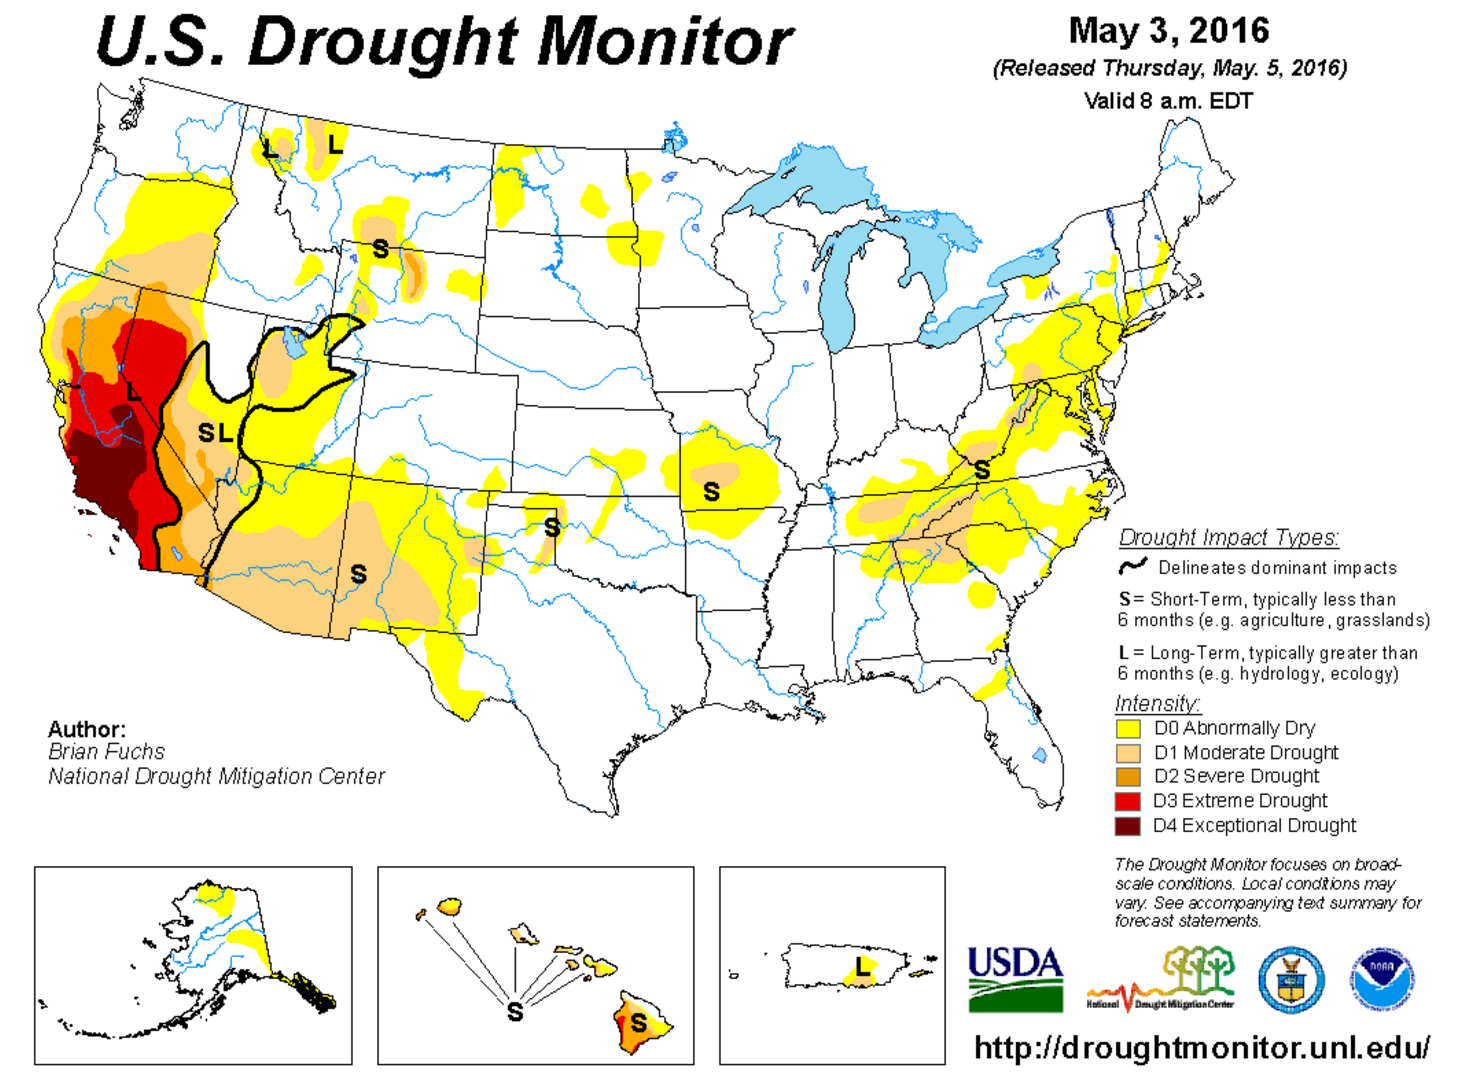
\includegraphics[width=0.8\textwidth]{figures/DroughtMonitor}
    \caption{}
\end{figure}

The drought in California demands particular attention given its severity and its impact on national food production. California grows about half of the US's fruit, nuts, and vegetables and 22\% of dairy \footnote{EPA State Agricultural Profiles, https://www3.epa.gov/region9/ag/ag-state.html}. It has been in severe drought for the past five years.  Currently, 90\% of the state is in drought.  More than 50\% is in severe to exceptional drought. \footnote{US Drought Monitor 2016.} Some towns in the Central Valley can no longer supply running water to all their residents. Some communities have undertaken dramatic mandatory water rationing, and Governor Jerry Brown has requested--and achieved--domestic water consumption decreases of around 25\%.    

But the welfare impacts on the people who live in drought-affected communities are not purely determined by the severity and duration of the drought. Low-income communities, like East Porterville in the CA Central Valley, are more likely to lose tap water than wealthy neighborhoods of Los Angeles.  This study sets out to identify the factors that predict how severely a drought will impact a community.  A better understanding of risk and resilience can support more effective policy to prevent and counteract the welfare impacts of drought.

\section{Data}
\begin{itemize} 
	\item Drought Monitor
	\\ The United States Drought Monitor combines a set of measures to categorize the severity of droughts in the US. Run in partnership between the National Drought Mitigation Center, the US Department of Agriculture, and the National Oceanic and Atmospheric Administration, a set of 250 experts reviews current data and revises the drought map every week. It was launched in 1999 to as an input for policymakers working on issues concerning water supply and drought.
	
	% YANG -- can you toss in a few bullet points here on the defintion of our drought variables?  I'll write them up into paragraphs
	\item NARR
	
	We use monthly temperature and precipitation from the NCEP North American Regional Reanalysis (NARR) project. 
	
	\item Yields
	
	We use annual, county-level crop yield data from the USDA for corn, soybeans, and wheat.
	
	\item Mortality
	
	We use county-level data from the CDC WONDER database for under-5, over-65, and all-ages mortality for 1999-2014. Metrics of mortality include total deaths, the crude mortality rate, and age adjusted mortality rates.

	\item ACS
	The American Community Survey is the annual survey conducted by the US Census. Data are available at the PUMA geographic level and are crosswalked to counties. Variables are weighted to represent the entire United States.  We use the ACS for demographic information such as population, age, race, and sex; employment and income information including employment in agriculture, annual household income, home ownership; and household water bills.

	\item Employment
	We use county-level data from the United States Bureau of Labor Statistics on the annual average total labor force, number employed, numer unemployed, and unemployment rate in each year of study.

	\item EPA
	
	We use geospatial data on facilities regulated by the United States Environmental Protection Agency to create a measure of the water intensiveness of the local economy.  We extract the FIPS code and the industrial category (SIC code) for each facility. Then we create a dummy variable for high water use and count the number of high-use facilities per county.

		The SICs that are coded high water- use are:
	
\begin{itemize}
\item Water-intensive industries:
\item 0100-0999 Agriculture, forestry, fishing
\item 2000-3999 Manufacturing
\item 4900-4932 Energy
	\end{itemize}
\end{itemize}	

There are several important issues with the use and interpretation of these data. We would like to clearly describe them up front. We decided to use the data despite these issues because it provided another opportunity to practice data management skills and because they may still provide some, albeit limited, insight.

First, these data are a snapshot of facilities managed in March, 2016. There is no way to gauge how the distribution of water-intensive industry has changed over time. This leads to two sample bias problems: first, the facilities contained in this data may not have existed during the window of our study. Second and most importantly, there may be an endogeneity problem where high water-use facilities in high-drought areas have shut down over the window of analysis and are missing from this sample. This would bias our estimates of the importance of water intensity down.

Finally, about two thirds of the observations had to be dropped due to a missing FIPS or SIC code. If this censoring is nonrandom, it introduces an additional source of bias to the study.

\item USDA Economic Research Service
	
	We use the Rural-Urban Continuum Codes from the USDA ERS to classify counties as rural or urban. Counties with a continuum code value greater than 3 are considered "non-metro" by the USDA ERS, and we code these as rural. All other counties are considered urban.

\section{Model}

We develop a two-stage model.  In the first stage, we estimate county-level "vulnerability" to drought by regressing key metrics of well-being on drought measures.  In the second stage, we identify predictors of vulnerability.

\begin{itemize}
	\textbf{Stage 1: Estimating vulnerability}

In the first stage, we run separate specifications with three dependent variables: the mortality rate, employment rate, and crop yields.  We select mortality and employment because they can be argued to paint a picture of a county's general well-being.  We select crop yields because they should respond strongly to drought, and give us insight into the salience of drought for agricultural versus non-agricultural communities.

Our model is as follows:

\begin{equation}
y_{i,t} = \beta_{i} D_{i,t} + \alpha_i + \tau_i t + \gamma_{s,t} + \epsilon_{i,t} \label{Eq1}
\end{equation}
where $D_{i,t}$ refers to the number of days in U.S. Drought Survey bins 2-4 in county $i$ and year $t$, $\alpha_i$ are county fixed effects controlling for time-invariant differences between counties, $\tau_i$ is the coefficient on a county level linear time trend, and $\gamma_{s,t}$ are state-by-year fixed effects controlling for state level time trends common across all counties $i \in s$. Note that the state-by-year fixed effects will non-parametrically account for national trends in the outcome of interest as well as state-level trends. The identifying variation in this model is within-county annual deviation from the county time trend and from statewide annual average drought levels. %We correct standard errors for serial correlation over space and time, due to the spatial and temporal nature of droughts (neighboring observations in time and space are not independent draws).
\\

 The coefficients from these regresssions indicate how responsive our measures of well-being -- mortality, employment, and crop yields -- are to drought.  These measures of vulnerability will be used as the dependent variables in the second stage. 

\item\textbf{Second Stage: Identifying the predictors of vulnerability}

What accounts for this variation in vulnerability to drought?  We use the vulnerability estiamtes from the first stage as dependent variables in the second stage.  We select a vector of potential predictors and test their statistical and economic significance.  These predictors include county-level socioeconomic characteristics such as racial composition, age distribution, income, monthly water bill, and measures of home ownership, rural v. urban, and water-intensiveness of the local economy.

The model is as follows:

\begin{equation}
\beta_i = \rho_0 + \boldsymbol{\delta} \mathbf{X}_i + \nu_i \label{Eq2}
\end{equation}

where the $\beta_i$ are the coefficients from (\ref{Eq1}) for a given outcome; $\mathbf{X}_i$ is a vector of county-level demographic and economic information; and $\boldsymbol{\delta}$ denote the associated coefficients.\\
~\\
This regression is cross-sectional and therefore not well identified from a causal perspective. Any omitted variable that happens to covary with both the levels of $\beta_i$ and the variables $\mathbf{X}_i$ will bias the coefficients $\boldsymbol{\delta}$. However, this model will illustrate how "drought resilience" (a low value of $\beta_i$) covaries with a set of common county socioeconomic characteristics. The goal with this stage is to build insight regarding what characteristics are commonly associated with drought vulnerability. % Because county level characteristics are likely to be correlated over space, we anticipate correcting our OLS standard errors by clustering over space.
\end{itemize}


\section{Discussion}

The results from the first stage are depicted in the following maps. Since we run several specifications of each regression, the clearest way to present our results is visually.  For tables of our full regression output, please reference the results folder on the git repository.

In the figure below, the colors represent the county-level correlation coefficients between three-year drought and corn yields, soybean yields, the elderly mortality rate, and unemployment,. We see comparable coefficients for corn and soy yields, with South Dakota, Indiana, and eastern North Carolina showing the most vulnerability to drought on soy yields and central Texas and southern Iowa showing the most vulnerability for corn.  Still, the coefficients are generally small, as we would expect given the impact of irrigation and other technological inputs on decoupling yields from weather outcomes.

The correlation between drought and unemployment is generally low, with Maine and Mississippi showing the greatest correlation. The correlation between drought and elderly mortality is stronger (the coefficient for any-age mortality is consistent, but weaker, as expected). Health and economics research shows strong effects of heat on mortality among the elderly in the absence of air conditioning. Future work should examine the impact of temperature and precipitation, rather than the composite drought measure, to see whether this effect is mainly driven by temperature or precipitation.

\begin{figure}[H]
	\centering
	\subfigure[Mortality]{%
		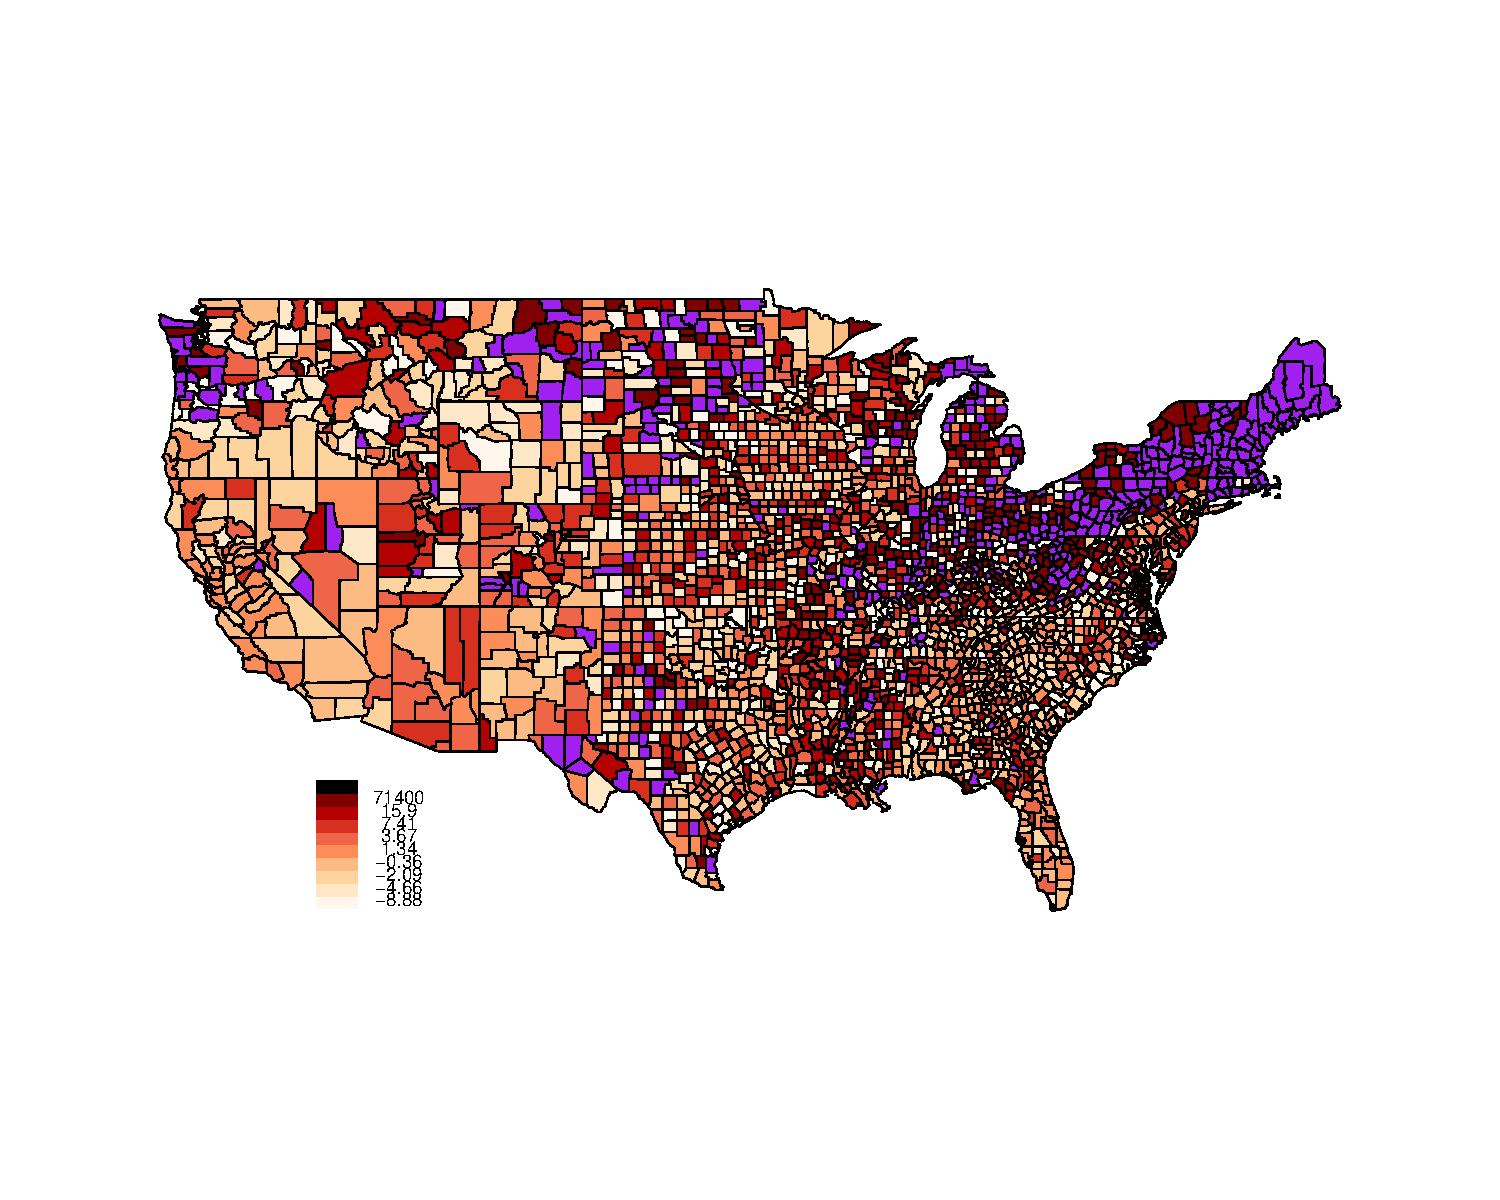
\includegraphics[width=0.4\textwidth]{shiny_screenshots/oldMortality3yrD}
		\label{fig:subfigure1}}
	\quad
	\subfigure[Unemployment]{%
		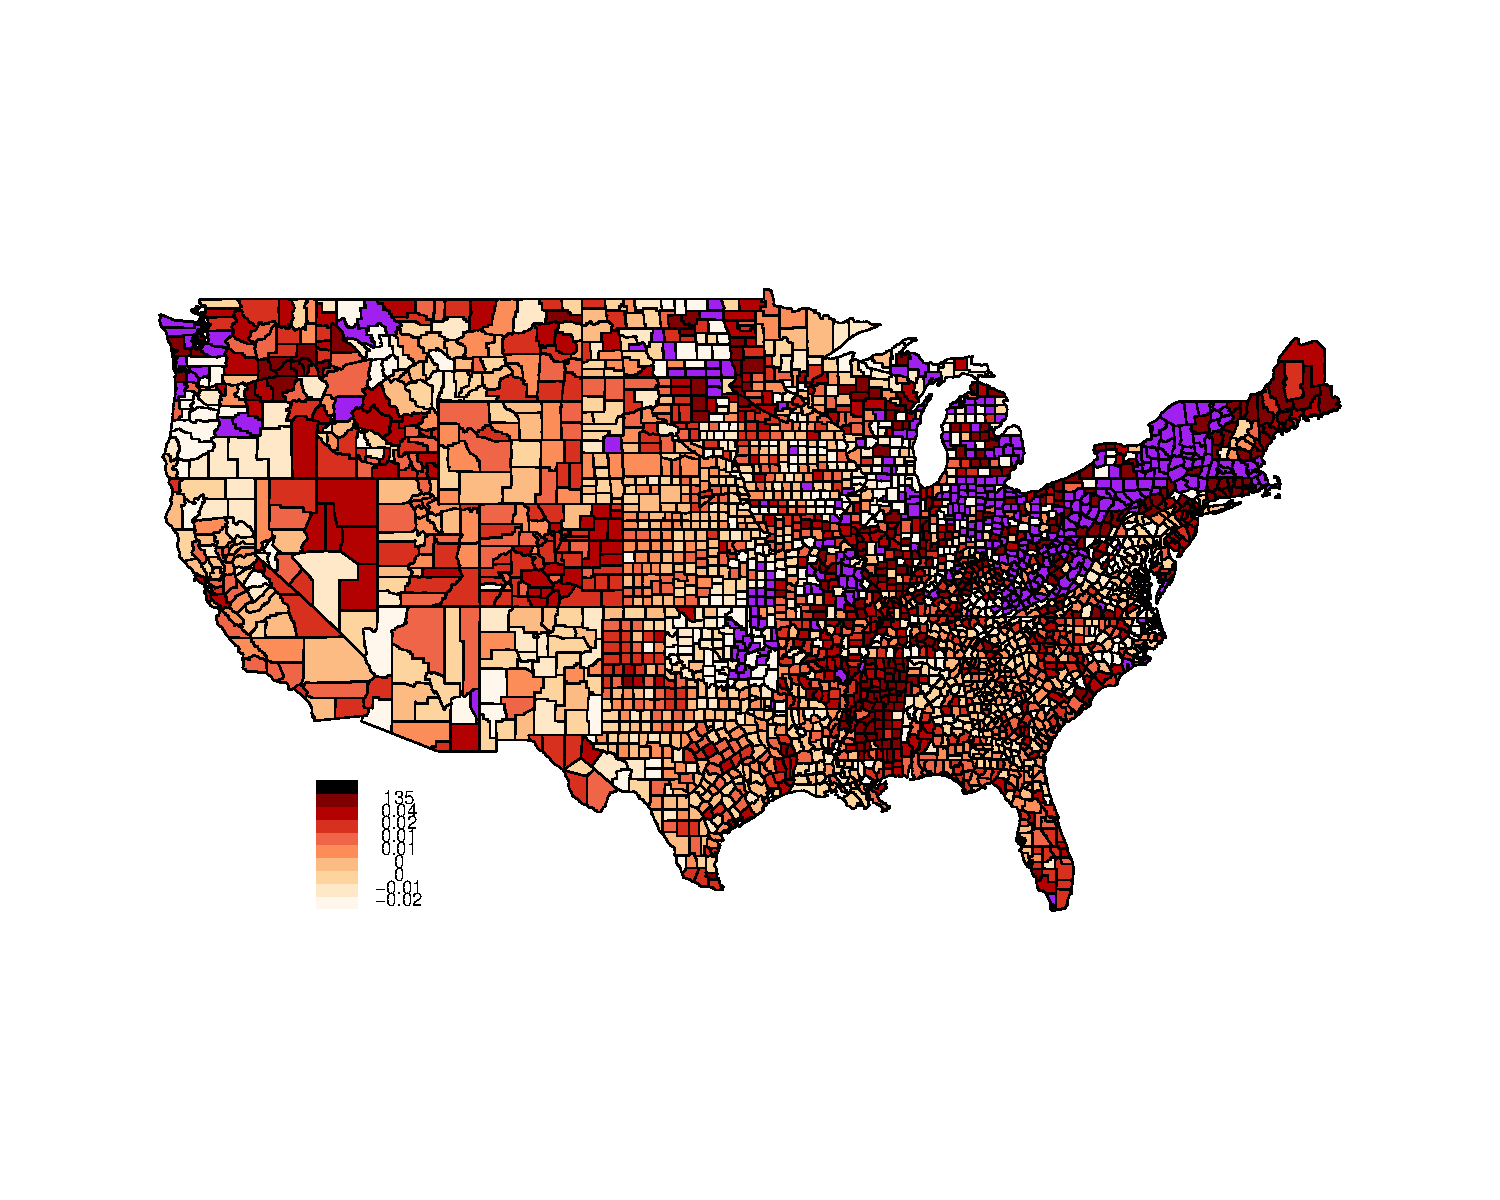
\includegraphics[width=0.4\textwidth]{shiny_screenshots/unemployment3yrD}
		\label{fig:subfigure2}}
	\subfigure[Corn]{%
		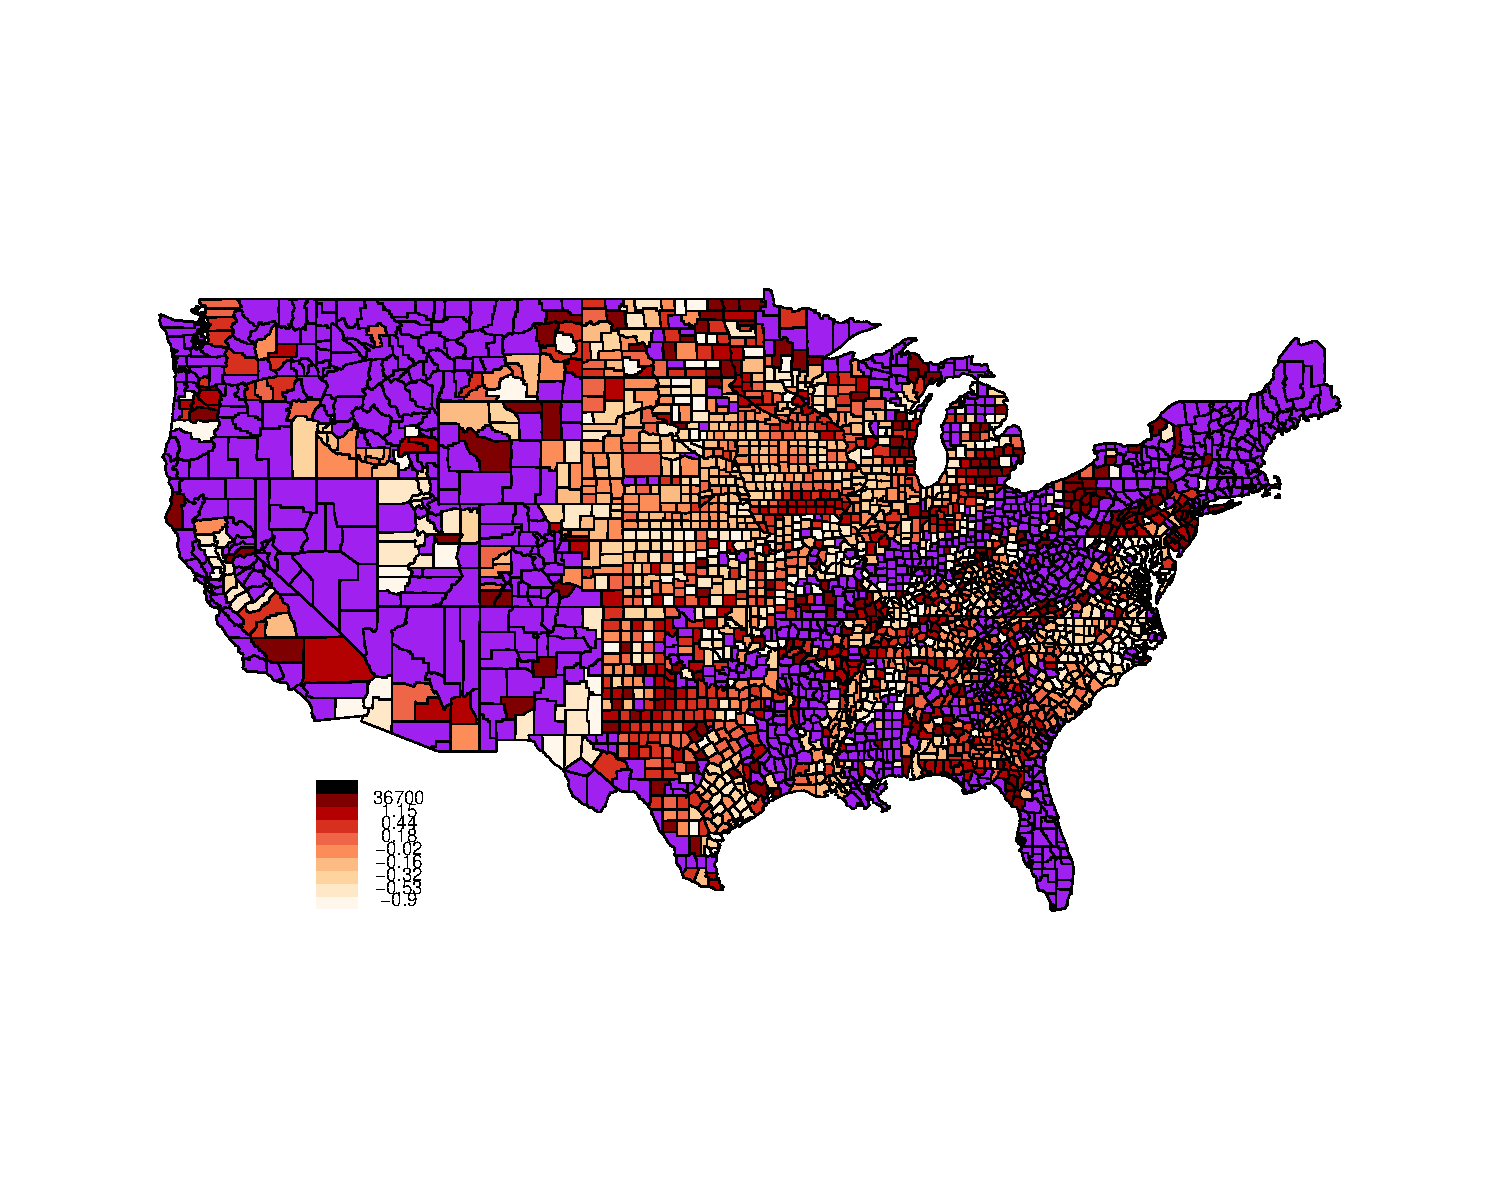
\includegraphics[width=0.4\textwidth]{shiny_screenshots/corn3yrDr}
		\label{fig:subfigure3}}
	\quad
	\subfigure[Soy]{%
		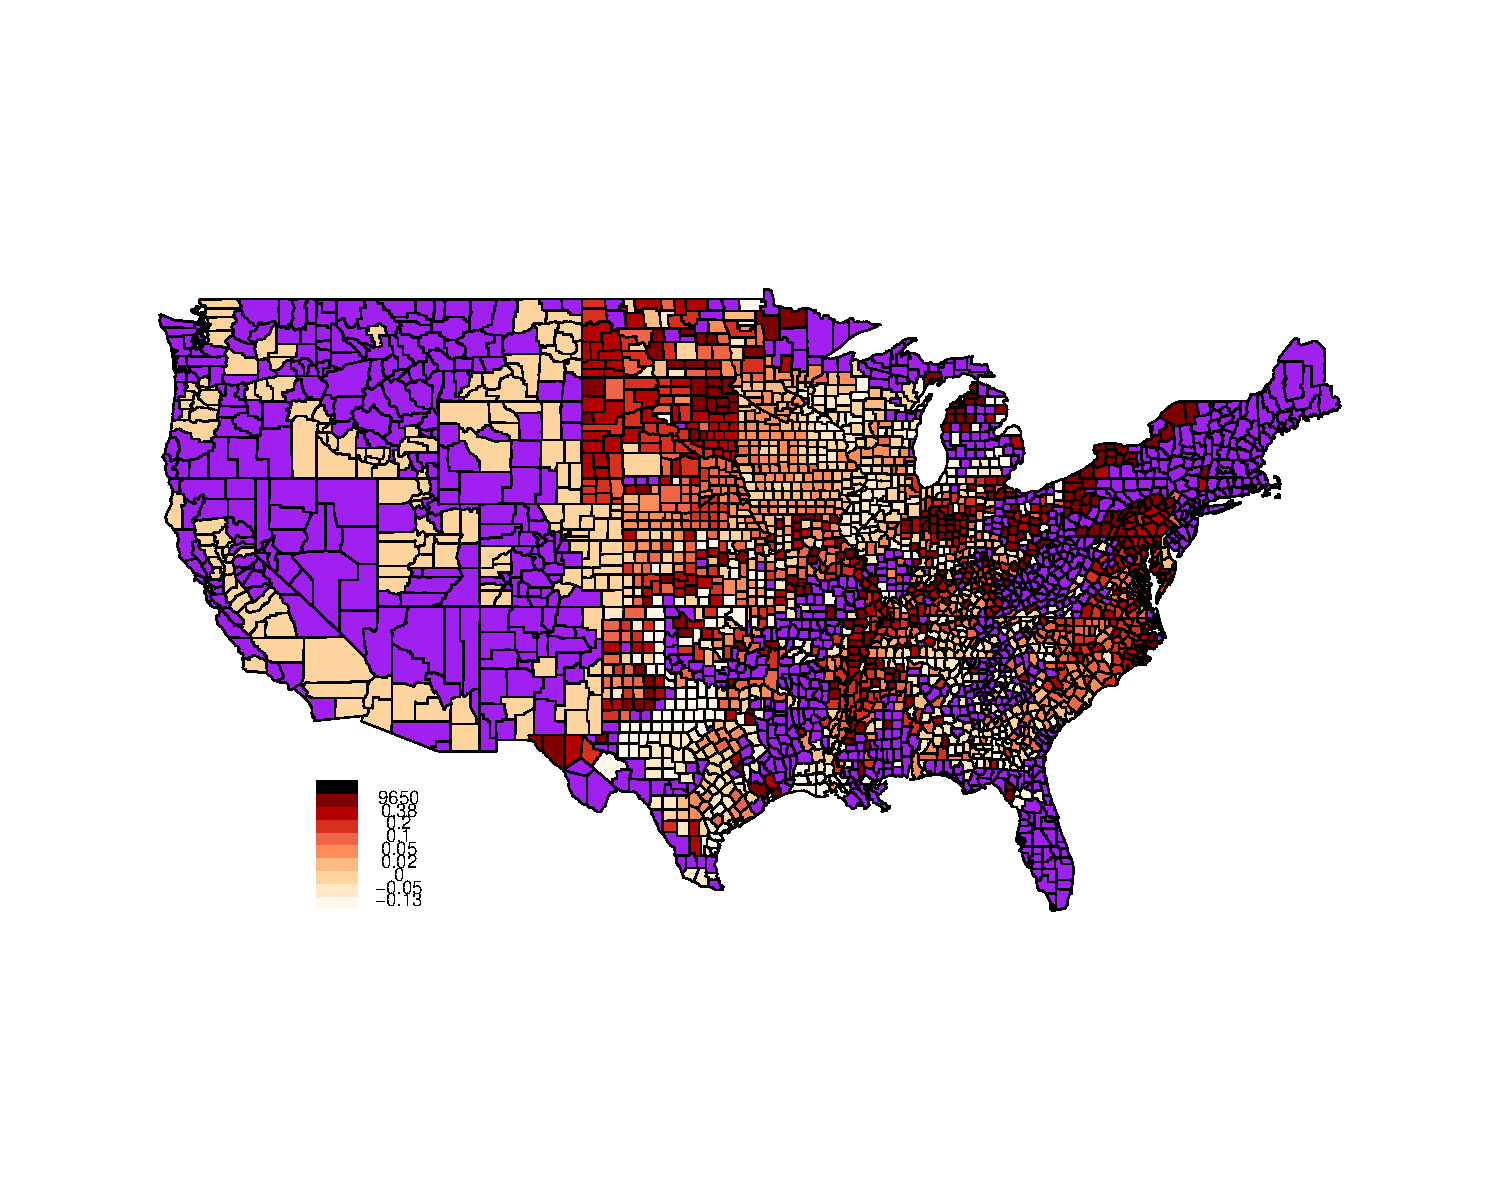
\includegraphics[width=0.4\textwidth]{shiny_screenshots/soy3yrD}
		\label{fig:subfigure4}}
	%
	\caption{First Stage Results}
	\label{fig:figure}
\end{figure}

In the second stage of analysis, we examine whether county-level demographic and economic characteristics predict the vulnerability to drought estimated in the first stage.  Our explanatory variables include demographic characteristics including percent white and percent Hispanic, age, and sex; and economic characteristics like percent of households who own their home, monthly water bill, percent employment in agriculture, and the water-intensiveness of the local economy.  

Full tables including the correlation coefficients and standard errors are available in the results folder on the git repository.  They are best explored through the Shiny app, which permits users to select specifications and immediately visualize results at the national and county levels.

Very few of the second-stage coefficients is statistically significant.  

\section{Conclusion}



\begin{thebibliography}{9}

\bibitem{employment}
U.S. Bureau of Labor Statistics.
\textit{Labor Force Data by County, Annual Averages}.
\\\texttt{http://www.bls.gov/lau/}
 
\bibitem{mortality} 
Center for Disease Control (CDC), U.S. Department of Health and Human Services. 
\textit{Mortality for 1999 - 2014 with ICD 10 codes}. 
\\\texttt{http://wonder.cdc.gov/mortSQL.html}

\bibitem{epa} 
Environmental Protection Agency (EPA). 
\textit{Facility Registry Service Spatial Data Download}. 
 \\\texttt{https://www.epa.gov/enviro/geospatial-data-download-service}
 
\bibitem{ACS} 
Missouri Census Data Center. \textit{American Communities Survey}.
\\\texttt{http://mcdc.missouri.edu/websas/geocorr14.html}

\bibitem{NARR}
National Centers for Environmental Prediction (NCEP). \textit{NCEP North American Regional Reanalysis}.
\\\texttt{http://www.esrl.noaa.gov/psd/}

\bibitem{DroughtMonitor} 
National Drought Mitigation Center (NDMC), U.S. Department of Agriculture (USDA), and the National Oceanic and Atmospheric Administration (NOAA). \textit{U.S. Drought Monitor}.
\\\texttt{http://droughtmonitor.unl.edu/}

\bibitem{rural}
United States Department of Agriculture, Economic Research Service. 2013 Urban-Rural Continuum Codes. \texttt{http://www.ers.usda.gov/data-products/rural-urban-continuum-codes.aspx}. Accessed 4/23/16.

\bibitem{yield}
United States Department of Agriculture, National Agricultural Statistics Service. Qick Stats. \texttt{https://quickstats.nass.usda.gov/}. Accessed 4/15/16.
 
\end{thebibliography}

\end{document}
